\begin{figure}[H]
  \centering\vspace{-0.3em}
  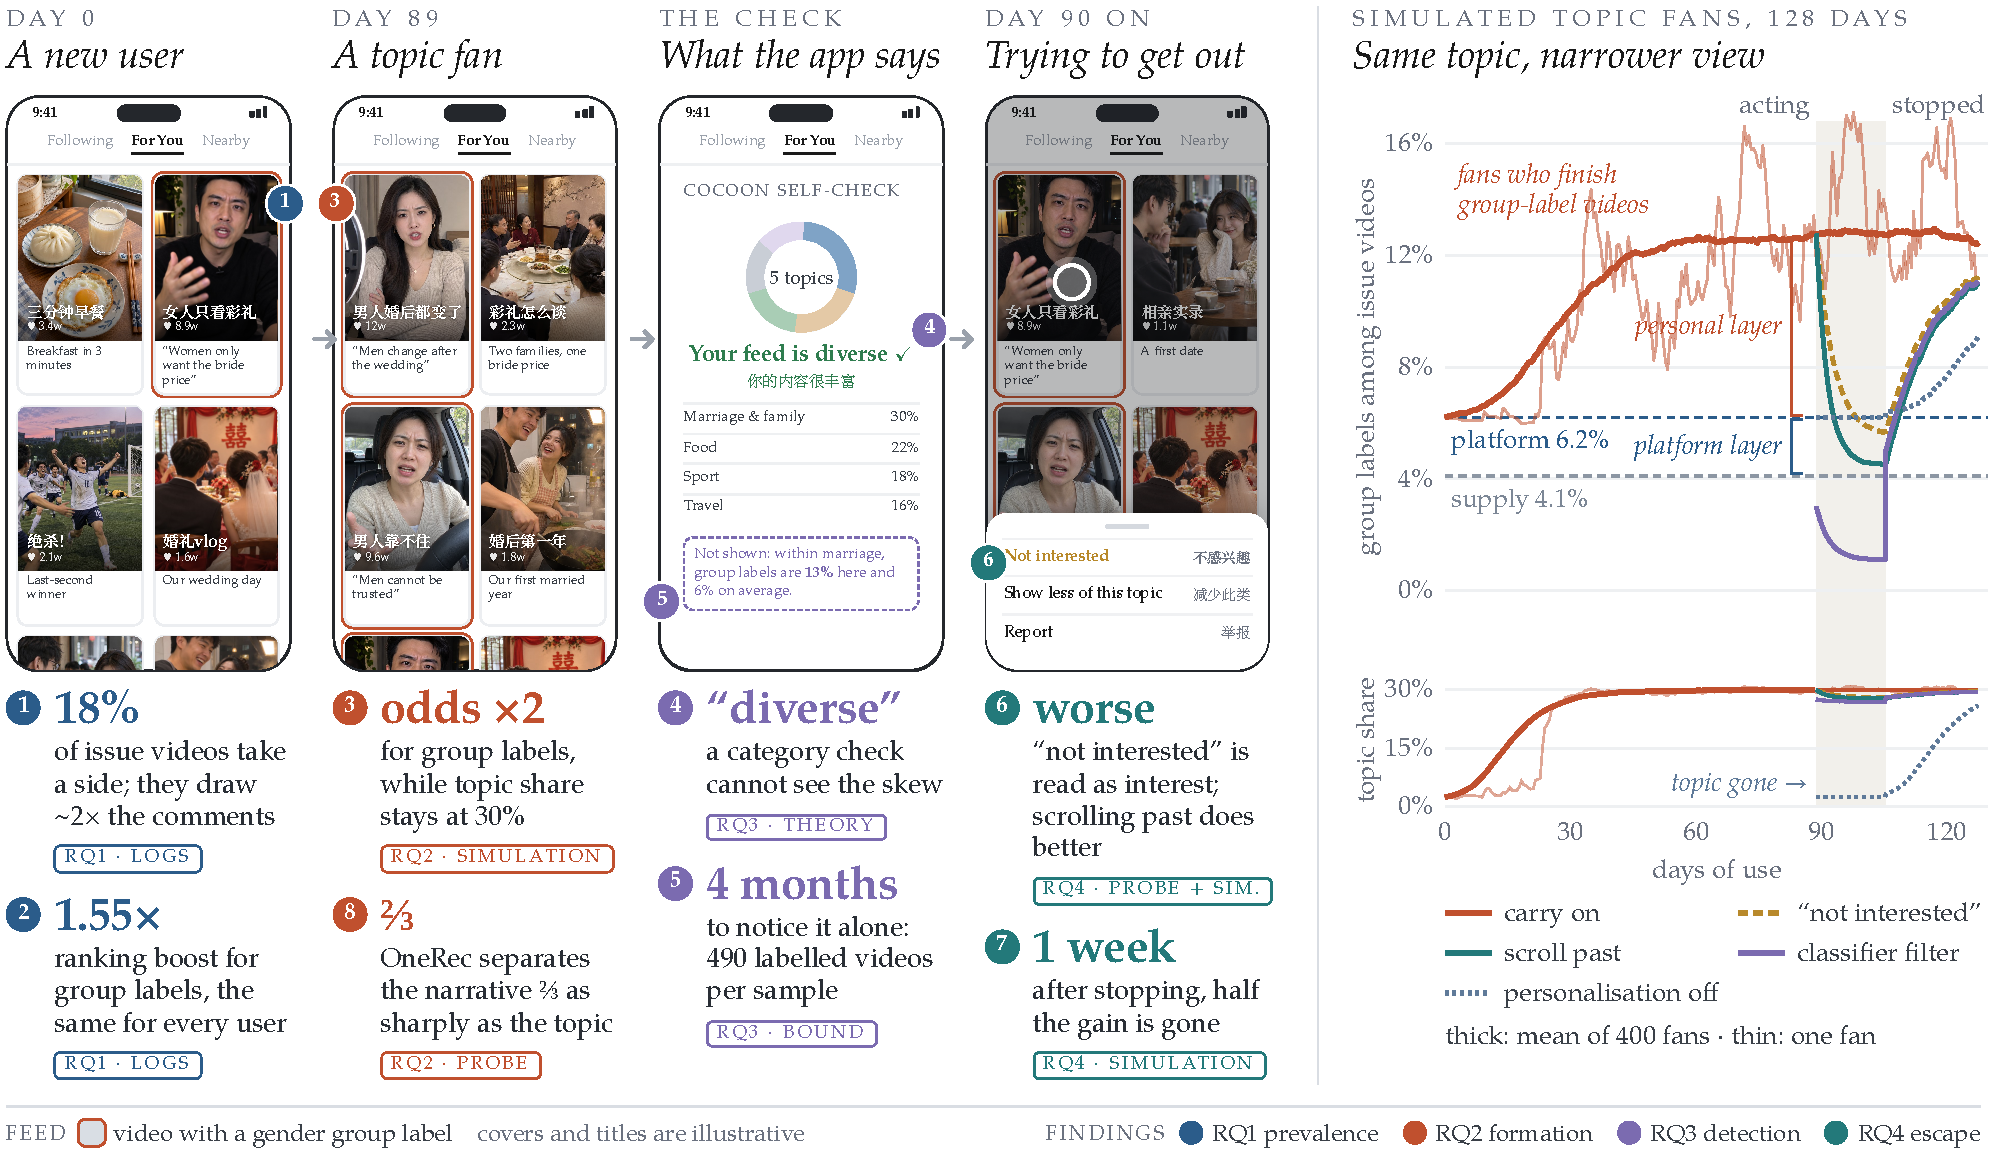
\includegraphics[width=\textwidth]{figures/fig_teaser.pdf}
  \caption{One user's 128 days and the four research questions. Ranking already shows gender group labels more often than they exist (\cnum{1}--\cnum{2}, RQ1). A fan of the topic who tends to finish them keeps the same topic share but doubles the odds of meeting them (\cnum{3}, \cnum{8}, RQ2). The app's category check calls the feed diverse, and noticing the skew alone takes months (\cnum{4}--\cnum{5}, RQ3). ``Not interested'' does worse than scrolling past, and gains fade once the user stops (\cnum{6}--\cnum{7}, RQ4). \textbf{Right:} simulated topic fans (\cref{sec:sim}), mean of 400 (thick) and one fan (thin). Feed screens are illustrative.}
  \label{fig:teaser}
\end{figure}

\section{Introduction}
\label{sec:intro}

A university student who opens a short-video app meets, between the cooking clips and the football highlights, a steady stream of arguments about how to live: whether to marry and whom, how a body should look, whether to sit the civil-service examination or go abroad, how much parents should decide, what is worth spending money on. Many of these videos do not inform so much as take a side. They present one choice as the only sensible one, or reduce a question to two camps, or attach a fault to an entire group of people. We call these \emph{opposing narratives}.

Public debate about such feeds is usually framed around the ``information cocoon''~\citep{sunstein2006infotopia} or ``filter bubble''~\citep{pariser2011filter}: the worry that a recommender shows people more and more of what they already like. Most research on the question, and the tools built in response to it, measure how narrow a feed is across \emph{topics} or content categories~\citep{nguyen2014exploring,li2022cocoon,sukiennik2024deep}. In 2025 Chinese platforms, after a national campaign against algorithm-related harms~\citep{cac2024qinglang}, launched self-assessments that tell users how concentrated their feed is over such categories~\citep{shiqi2025kuaishou}.

A measure over topics has a blind spot, illustrated in \cref{fig:teaser}. Two users may both give a third of their feed to marriage videos. The first sees the usual range of stories, advice and jokes. The second sees, within the same topic, twice as many videos saying that women only care about money or that men cannot be trusted. A topic-level check gives both the same score. If either has a problem it is the second user, who may be perfectly happy with the topic itself and have no wish to see less of it. That feed has kept the topic and narrowed the view. We call this a \emph{viewpoint cocoon}.

Audits of platforms at the level of viewpoints do exist, but they treat political ideology or misinformation on YouTube and TikTok, and observe the platform from outside~\citep{haroon2023youtube,hosseinmardi2024bots,pecher2026tiktok}. Studies of user controls report how much unwanted content a button removes, not how much wanted content goes with it~\citep{ricks2022button,liu2024train,kaplan2026foryou}. To our knowledge, no study separates viewpoint skew within an everyday issue from interest in that issue, and then follows the skew from formation to detection to escape. This report does so, guided by four questions.

\begin{rqbox}
\small
\begin{description}[leftmargin=3.2em,style=sameline,itemsep=0.2em,topsep=0pt]
  \item[\RQ{1}] \textbf{Prevalence.} Across the everyday issues in a short-video feed, how common are opposing narratives, and of which types? Do they draw more engagement, and does ranking show them more often than they occur among the videos available?
  \item[\RQ{2}] \textbf{Formation.} For a user who tends to finish one narrative, how far and how fast does personalisation tilt the mix within the topic?
  \item[\RQ{3}] \textbf{Detection.} How many videos must the user count before such a tilt can be told from chance?
  \item[\RQ{4}] \textbf{Escape.} How much does each action open to the user reduce the tilt, at what cost in lost topic and effort, and for how long? Which part of the tilt can no user action reach?
\end{description}
\end{rqbox}

We answer them on public data from Kuaishou: the RecIF interaction logs and OneRec, an open generative recommender trained on those logs~\citep{zhou2025openonerec}. RQ1 covers five issue domains; RQ2--RQ4 follow one narrative in depth, videos that attach a negative label to a whole gender, because gender and marriage is the domain with the most opposing narratives and group labels are the sharpest of them. Each question draws on the evidence best suited to it (\cref{fig:overview}): language-model labels of the logs for RQ1, the logs together with controlled edits of the histories given to OneRec and a simulation fitted to those edits for RQ2, a sample-size bound for RQ3, and the simulation for RQ4. The report makes five contributions.

\begin{enumerate}
  \item \textbf{A definition that separates interest from skew} (\cref{sec:framework}). A feed is described by its topic share $m$ and its viewpoint skew $V$; total skew splits exactly into a platform layer and a personal layer, and five propositions state what feedback, topic controls and filters can change and how many videos detection needs.
  \item \textbf{A map of opposing narratives} (\cref{sec:data}). They carry \nOppShare\% of issue impressions, draw more engagement, and are shown more often than they occur among the videos available.
  \item \textbf{Evidence on formation from three sources} (\cref{sec:formation}). Logs, recommender probes and a fitted simulation agree that OneRec separates the narrative about two-thirds as sharply as the topic; in simulation this doubles a fan's odds of meeting it within three months.
  \item \textbf{A bound on noticing} (\cref{sec:detection}). Telling a doubling from chance takes about \nDetNDouble{} labelled issue videos in each of two samples, four months of viewing for the reference sample.
  \item \textbf{A price list for escape} (\cref{sec:escape}). In simulation, topic-level settings remove the skew only with the topic, ``not interested'' does worse than scrolling past, and once old habits return, the gains that keep the topic halve within about a week.
\end{enumerate}
